\chapter{L'interdiction favorise-t-elle la criminalité ?}

	\section{La prohibition: un terreau pour le développement des réseaux criminels}

\paragraph{Un débat relancé}

    La légalisation du cannabis est un sujet récurrent et régulièrement débattu, notamment par les politiques. Le 11 avril 2016, Jean-Marie Le Guen n’a pas fait exception en relançant le débat \cite{leguen16}. L’un de ses arguments étant que légaliser le cannabis baisserait la criminalité. En effet, en 2014, 10 \% des dossiers judiciaires concernaient la drogue et plus précisément 91 \% d’entre eux étaient liés au cannabis, le plus souvent à sa consommation. C’est pourquoi, une légalisation ou décriminalisation entraînerait une chute de la criminalité. Cependant, cette diminution ne serait absolument pas liée à une baisse de la consommation de cannabis. On ne peut donc pas vraiment considérer cela comme une solution au problème de la consommation du cannabis.

\paragraph{Le syndrome de la vitre cassée}

    En revanche, le syndrome de la vitre cassée implique une baisse de la criminalité.

    Le syndrome de la vitre cassée est une théorie parue et développée dans un ouvrage de Georges Kelling, un criminologue du New Jersey. Selon lui \cite{wikiVitreBrisee}, si on prend l’exemple d’un quartier résidentiel, le délabrement des bâtiments, notamment visible par une vitre brisée (d’où le nom), encouragerait à la criminalité et au dépravement. En effet, constater que les bâtiments ne sont pas entretenus, que les gens ne sont pas forcément très polis entre eux, donne un sentiment d’impunité et augmente par la même le nombre de petits délits. Ceux ci ne semblent plus très importants, au vue de l’environnement. Certaines personnes se sentent donc moins coupables, ont moins l’impression de faire quelque chose de mal et c’est ainsi que le taux de criminalisation augmente. Le fait de voir beaucoup de criminalité renforce le sentiment qu’on peut faire des choses illégales et augmente la criminalité. C’est ce cercle vicieux qu’on appelle le syndrome de la vitre cassée.

\begin{figure}\centering
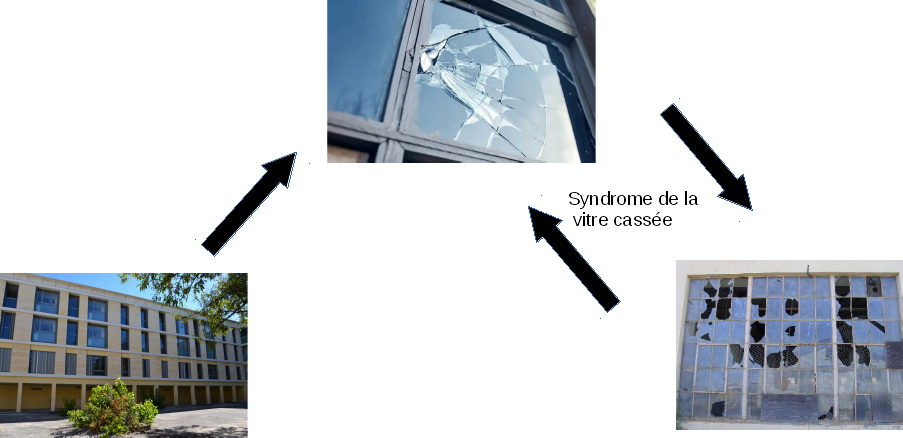
\includegraphics[width=.8\textwidth]{images/vitrecassee.png}
\caption{Schéma d’explication du syndrome de la vitre cassée}
\end{figure}

    En reprenant l’exemple du cannabis, une légalisation permettrait effectivement de diminuer la criminalité, et pas seulement celle liée à la détention, la consommation ou la vente. En supprimant quasiment 140 000 infractions par an, la criminalité est moins exposée aux yeux de tous, notamment ceux des plus jeunes, donnant une impression plus reluisante de notre société et dissuadant ainsi des possibles criminels qui se sentiront plus « encadrés ».

    En admettant qu’une légalisation du cannabis permettrait de diminuer la criminalité, elle libèrerait par la même occasion une quantité non négligeable de places dans les prisons.
    

\section{Les prisons surpeuplées : une culture lucrative}

\paragraph{Pourquoi une privatisation des prisons ?}

    Suite à une surpopulation carcérale et de manière générale à des restrictions des budgets publics, il y a une trentaine d’années, un phénomène partant des États Unis mais se répandant très vite à travers le monde est apparu : les prisons privées. Cette privatisation prend deux formes : la privatisation totale et la gestion mixte.

    La privatisation totale \cite{dufresne10}, comme son nom l’indique est totale. L’entreprise privée assure donc toute la prise en charge de la prison, de sa construction à la surveillance des détenus. Ce type de prison n’est cependant pas présent en France, même si il reste utilisé aux États-Unis, au Royaume Unis ainsi qu’en Australie.

    La gestion mixe, aussi nommée Partenariat Public Privé, concerne les prisons dans lesquelles l’État a un réel contrôle. Il délègue cependant une partie de son pouvoir à certaines entreprises privées. Ces contrats s’étendent sur au moins 25 ans à partir de l’ouverture de la prison


\paragraph{La situation en France}

    La privatisation des prisons en France, si elle s’étend de plus en plus, a commencé de manière progressive avec la loi Chalandon en 1987, puis s’est renforcée avec la loi d’orientation et de programmation judiciaire de 2002. Ainsi, l’État doit obligatoirement conserver quelques tâches comme la surveillance des prisons ou la direction des prisons. Les autres tâches, ne nécessitant pas un pouvoir particulier, sont de plus en plus assurées par des entreprises privées. Au début, seules la conception et la réalisation des prisons étaient concernées par cette privatisation. L’État paye bien évidemment les entreprises pour les tâches qu’elles accomplissent, allant même jusqu’à leur verser un loyer proportionnel au coût de fabrication des bâtiments.

    Selon l’observatoire des multinationales, en 2016, 68 prisons étaient privées pour un total de 188 prisons. Cela représente environ 36 \% des prisons. De plus, plus de la moitié des prisonniers sont détenus dans des prisons privées. Les entreprises profitant de ce marché n’ont donc pas intérêt à ce qu’un nombre important de peines soient réduites, ou même supprimées comme cela serait le cas avec la légalisation du cannabis.

    Depuis 2008, nous somme entrés dans le type de privatisation évoqué précédemment : le partenariat public-privé. Selon l’Organisation Internationale des Prisons (OIP) \cite{knaebel16}, avec ces contrats, l'Etat doit verser en loyer environ 5,9 milliards d’euros par an. De plus, après s’être engagé à payer un loyer pour les 25 années à venir, l’État n’a aucun intérêt à réduire des peines ou à vider les prisons maintenant. 

    
\section{Le marché noir : une vitrine sur les drogues}

\paragraph{Un marché noir très présent}

    Actuellement, consommation, production et possession de cannabis ou autres drogues sont interdites (sauf pour raisons médicales). Comme toute interdiction, celle ci favorise le développement d’un marché noir et de toute une organisation criminelle comprenant gangs, dealer, etc. Cela représente une part de la criminalité

\paragraph{Le cannabis : une drogue d’introduction}

    Avec cette forte présence du marché noir, il est devenu facile de se procurer du cannabis. Si cette drogue appartient à la catégorie des drogues douces, ce n’est pas le cas de toutes les drogues vendues par le dealer auprès de qui les consommateurs se fournissent. C’est pourquoi, l’interdiction du cannabis peut d’une certaine façon donner un nouveau rôle à cette drogue : une drogue d’introduction.

    Quand le consommateur rentre en contact avec un dealer, celui-ci lui vend ce qu’il demande. Seulement à partir d’un certain temps, le consommateur peut, par curiosité ou pour d’autres raisons, s’intéresser à des drogues dures, plus dangereuses. De plus, on peut ici aussi appliquer le syndrome de la vitre cassée (expliqué dans la partie I.1). En effet, le consommateur étant déjà dans l’illégalité en achetant et consommant le cannabis, il ne verra pas de grande différence entre le cannabis et les autres drogues que peut lui fournir le dealer. À titre d’exemple sur une situation à peu près équivalente, aux États-Unis lors de l’interdiction de la consommation d’alcool, celle ci était devenue incontrôlable. 

%Transition :
On remarquera aussi que si une légalisation mettrait en échec le marché noir, ce n’est pas le cas d’une dépénalisation qui interdit toujours la vente.
